\section{Overview}
In this section, we will explain the overall structure of Germinate along with an overview of the various data types that Germinate supports.

\subsection{Authentication}
Germinate can be used with or without user authentication. If the administrator of Germinate decided to enable authentication, you will be asked to log in using a username and password. Figure \ref{fig:overview:login} shows the login page of Germinate. If you already have a user account, simply enter the username and password into the provided text boxes.

If you do not have a user account, click on the link below the login button to create an account. You may get asked to agree to a license agreement before being able to create an account.

\begin{figure}
	\centering
	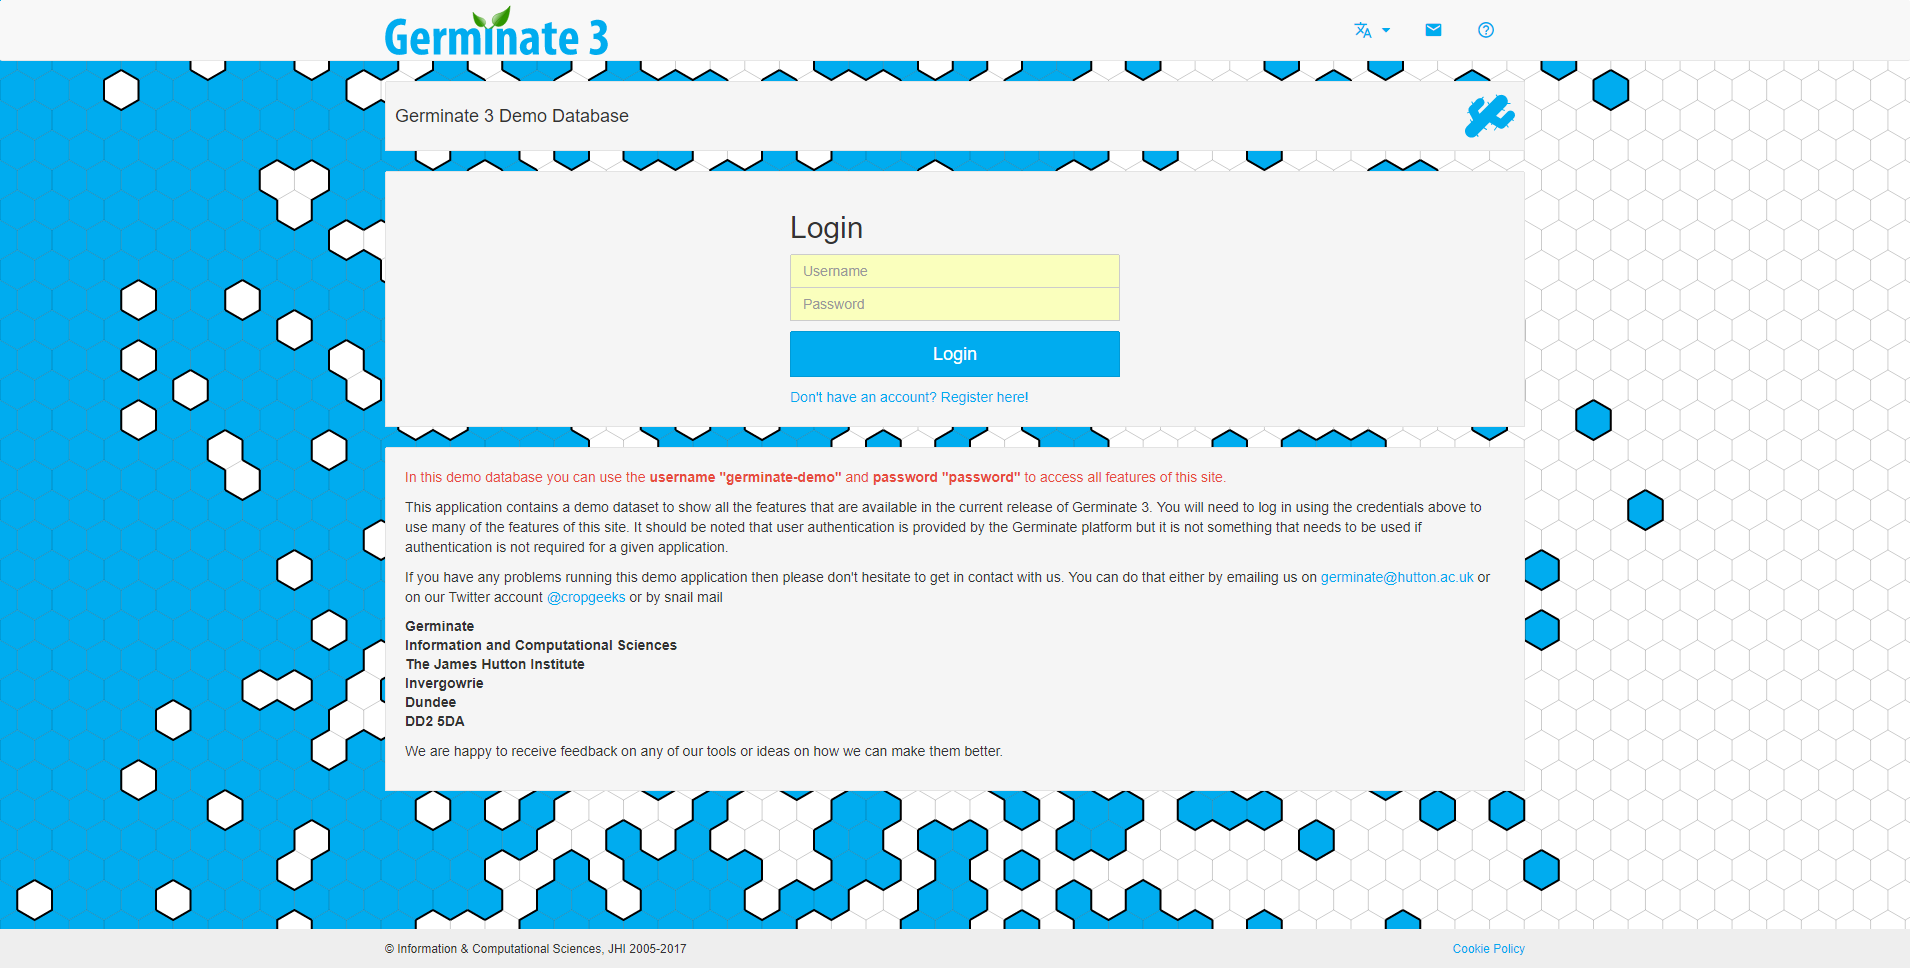
\includegraphics[width=0.85\linewidth]{img/overview/login.png}
	\caption{Depending on the configuration of Germinate, you may be asked to log in.}
	\label{fig:overview:login}
\end{figure}

\subsection{Page layout}
Figure \ref{fig:overview:home} shows the main layout of the Germinate web interface. The interface has a banner along the top containing the Germinate logo and a few dropdown menu items in the top right corner (c.f. Figure \ref{fig:overview:home}C). These items include the language selector which will be covered in Section \ref{sec:features:language-selector}, social media buttons, the marked item lists covered in Section \ref{sec:features:marked-items}, a user menu with specific functions based on your type of account and, finally, a help button that can be clicked to get more information about the current page (c.f. Section \ref{sec:features:help}).
\todo{Explain and reference other elements from figure 2}

\begin{figure}
	\centering
	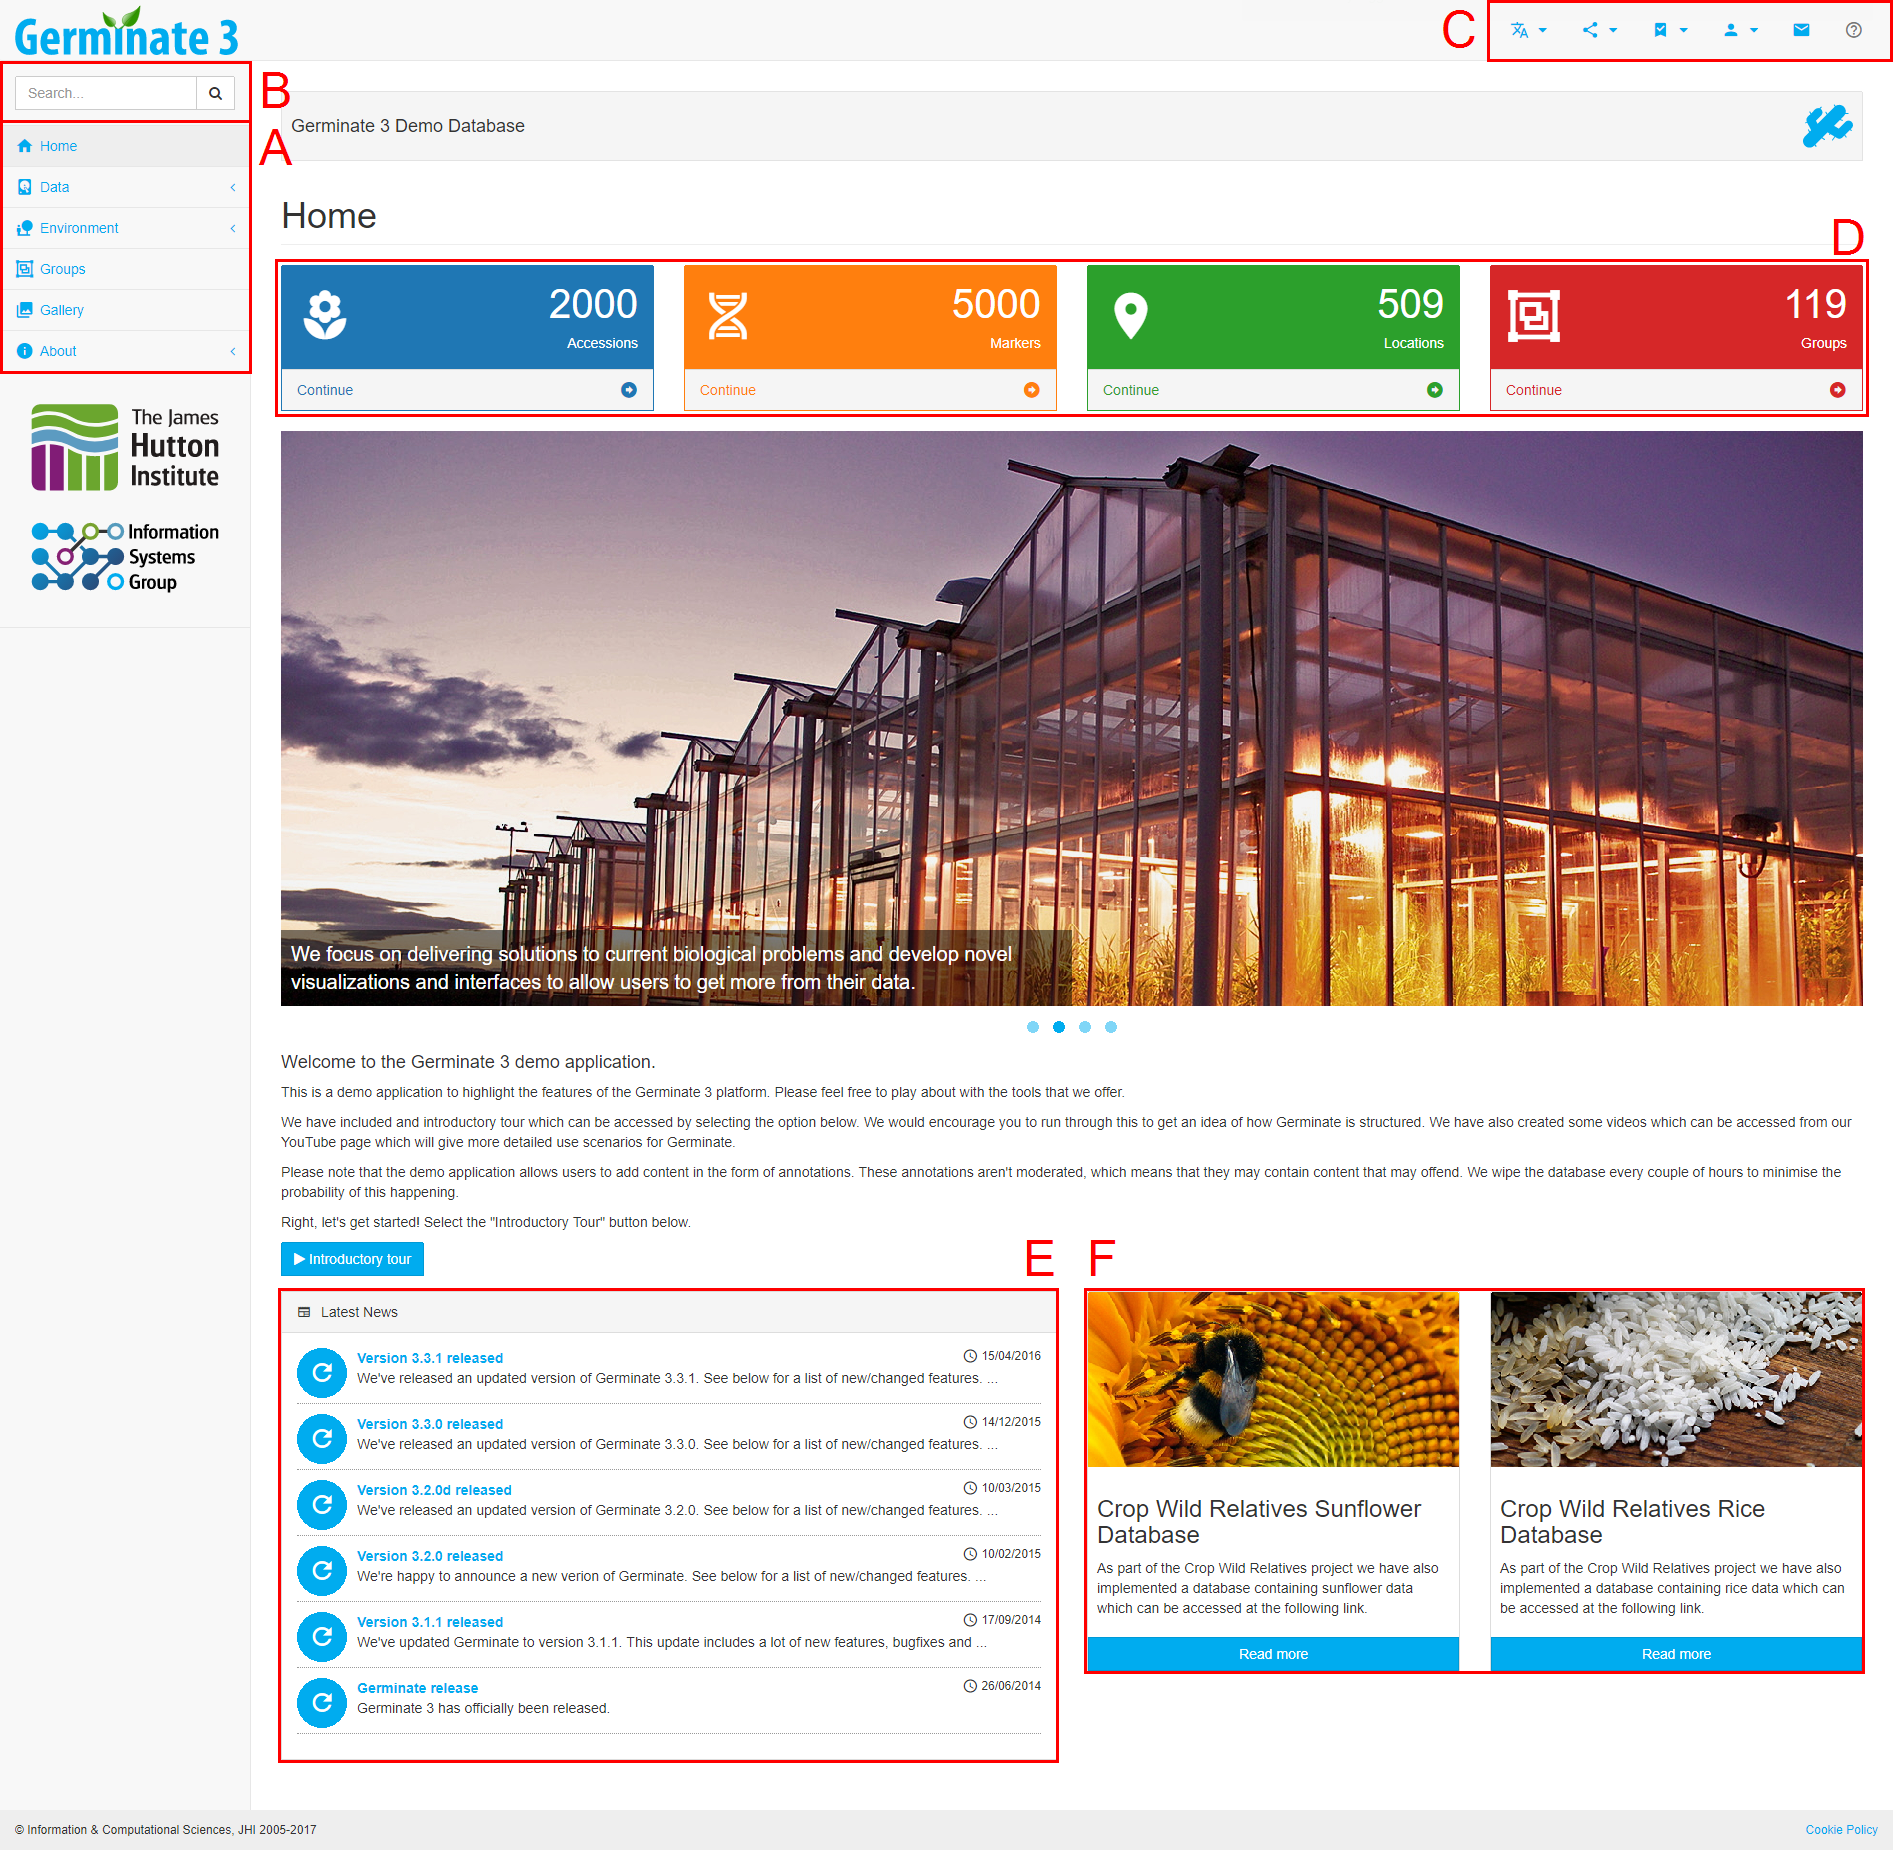
\includegraphics[width=0.85\linewidth]{img/overview/home.png}
	\caption{The home page of Germinate is the first page you will see. (A) The main menu of Germinate used to navigate the page. (B) The search box used for free-text searches of the database. (C) Language selector, social media buttons, marked item lists, user menu and the help button. (D) Latest news about this instance of Germinate and the contained data.}
	\label{fig:overview:home}
\end{figure}